\documentclass[spanish,a4paper,11pt,twoside]{report}

%%%%%%%%%%%%%%%%%%%%%%%%%%%%%%%%%%%%%%%%%%%%%%%%%%%%%%%%%%%%%%%%%%%%%%%%%%%%%%%
\usepackage[dvips]{graphicx}
\usepackage[dvips]{epsfig}
\usepackage[latin1]{inputenc}
\usepackage[spanish]{babel}
\usepackage{alltt}
\usepackage{templates/algorithm}
\usepackage{templates/algorithmic}
\usepackage{templates/multirow}

%%%%%%%%%%%%%%%%%%%%%%%%%%%%%%%%%%%%%%%%%%%%%%%%%%%%%%%%%%%%%%%%%%%%%%%%%%%%%%%

\newcommand{\SONY}{{\sc Sony}}
\newcommand{\MICROSOFT}{{\sc Microsoft}}
\newcommand{\GCC}{\textsf{\textsc{G}CC}}
\newcommand{\INTEL}{\textsf{\textsc{I}ntel}}

%%% Traducimos el pseudocodigo
\renewcommand{\algorithmicwhile}{\textbf{mientras}}
\renewcommand{\algorithmicend}{\textbf{fin}}
\renewcommand{\algorithmicdo}{\textbf{hacer}}
\renewcommand{\algorithmicif}{\textbf{si}}
\renewcommand{\algorithmicthen}{\textbf{entonces}}
\renewcommand{\algorithmicrepeat}{\textbf{repetir}}
\renewcommand{\algorithmicuntil}{\textbf{hasta que}}
\renewcommand{\algorithmicelse}{\textbf{en otro caso}}
\renewcommand{\algorithmicfor}{\textbf{para}}

%\newcommand{\RETURN}{\textbf{retornar} }
\newcommand{\RET}{\STATE \textbf{retornar} }
\newcommand{\TO}{\textbf{hasta} }
\newcommand{\AND}{\textbf{y} }
\newcommand{\OR}{\textbf{o} }

%%%%%%%%%%%%%%%%% Creamos un entorno para listar c�digo fuente %%%%%%%%%%%%%%%
\newenvironment{sourcecode}
{\begin{list}{}{\setlength{\leftmargin}{1em}}\item\scriptsize\bfseries}
{\end{list}}

\newenvironment{littlesourcecode}
{\begin{list}{}{\setlength{\leftmargin}{1em}}\item\tiny\bfseries}
{\end{list}}

\newenvironment{summary}
{\par\noindent\begin{center}\textbf{Abstract}\end{center}\begin{itshape}\par\noindent}
{\end{itshape}}

\newenvironment{keywords}
{\begin{list}{}{\setlength{\leftmargin}{1em}}\item[\hskip\labelsep \bfseries Keywords:]}
{\end{list}}

\newenvironment{palabrasClave}
{\begin{list}{}{\setlength{\leftmargin}{1em}}\item[\hskip\labelsep \bfseries Palabras clave:]}
{\end{list}}


%%%%%%%%%%%%%%%%%%%%%%%%%%%%%%%%%%%%%%%%%%%%%%%%%%%%%%%%%%%%%%%%%%%%%%%%%%%%%%%
% Format
%%%%%%%%%%%%%%%%%%%%%%%%%%%%%%%%%%%%%%%%%%%%%%%%%%%%%%%%%%%%%%%%%%%%%%%%%%%%%%%

%%\topmargin -4 mm
%\topmargin -21 mm
%\headheight 10 mm
%\headsep 10 mm

%\textheight 229 mm
%\textheight 246 mm

%\oddsidemargin -5.4 mm
%\evensidemargin -5.4 mm
\oddsidemargin 5 mm
\evensidemargin 5 mm

%\oddsidemargin -3 mm
%\evensidemargin -3 mm

%\textwidth 17 cm
\textwidth 15 cm
%\columnsep 10 mm

\input{amssym.def}

%%%%%%%%%%%%%%%%%%%%%%%%%%%%%%%%%%%%%%%%%%%%%%%%%%%%%%%%%%%%%%%%%%%%%%%%%%%%%%%

\begin{document}

%%%%%%%%%%%%%%%%%%%%%%%%%%%%%%%%%%%%%%%%%%%%%%%%%%%%%%%%%%%%%%%%%%%%%%%%%%%%%%%
% First Page 
%%%%%%%%%%%%%%%%%%%%%%%%%%%%%%%%%%%%%%%%%%%%%%%%%%%%%%%%%%%%%%%%%%%%%%%%%%%%%%%

\pagestyle{empty}
\thispagestyle{empty}


\newcommand{\HRule}{\rule{\linewidth}{1mm}}
\setlength{\parindent}{0mm}
\setlength{\parskip}{0mm}
\vspace*{\stretch{1}}

\begin{center}
\includegraphics[width=0.2\textwidth]{images/logotipo-secundario-ULL}\\[0.25cm]
\end{center}

\HRule
\begin{center}
        {\Huge SERIES NUM�RICAS} \\[2.5mm] 
        {\Huge Funci�n trigonom�trica: sin(x)} \\[2.5mm]
        {\Large Jorge Antonio Herrera Alonso\\[5mm]
		 Elizabeth Hern�ndez Mart�n\\[5mm]
		 Yessica Sabrina G�mez Buso}\\[5mm]
        {\Large \textit{Grupo ($2\mid F$) }} \\[5mm]


        {\em T�cnicas Experimentales. $1^{er}$ curso. $2^{do}$ semestre} \\[5mm]
        Lenguajes y Sistemas Inform�ticos \\[5mm]
        Facultad de Matem�ticas \\[5mm]
        
        Universidad de La Laguna \\
\end{center}
\HRule
\vspace*{\stretch{2}}
\begin{center}
  La Laguna, \today 
\end{center}

%%%%%%%%%%%%%%%%%%%%%%%%%%%%%%%%%%%%%%%%%%%%%%%%%%%%%%%%%%%%%%%%%%%%%%%%%%%%%%%

%%%%%%%%%%%%%%%%%%%%%%%%%%%%%%%%%%%%%%%%%%%%%%%%%%%%%%%%%%%%%%%%%%%%%%%%%%%%%%%
\newpage{\pagestyle{empty}\cleardoublepage}

\pagestyle{myheadings} %my head defined by markboth or markright
% No funciona bien \markboth sin "twoside" en \documentclass, pero al
% ponerlo se dan un mont�n de errores de underfull \vbox, con lo que no se
% ha puesto.
\markboth{Jorge Herrera, Elizabeth Hern�ndez, Yessica G�mez}{Series Num�ricas}

%%%%%%%%%%%%%%%%%%%%%%%%%%%%%%%%%%%%%%%%%%%%%%%%%%%%%%%%%%%%%%%%%%%%%%%%%%%%%%%
%Numeracion en romanos
\renewcommand{\thepage}{\roman{page}}
\setcounter{page}{1}

%%%%%%%%%%%%%%%%%%%%%%%%%%%%%%%%%%%%%%%%%%%%%%%%%%%%%%%%%%%%%%%%%%%%%%%%%%%%%%%

\tableofcontents

%%%%%%%%%%%%%%%%%%%%%%%%%%%%%%%%%%%%%%%%%%%%%%%%%%%%%%%%%%%%%%%%%%%%%%%%%%%%%%%
\newpage{\pagestyle{empty}\cleardoublepage}

\listoffigures

%%%%%%%%%%%%%%%%%%%%%%%%%%%%%%%%%%%%%%%%%%%%%%%%%%%%%%%%%%%%%%%%%%%%%%%%%%%%%%%
\newpage{\pagestyle{empty}\cleardoublepage}

\listoftables

%%%%%%%%%%%%%%%%%%%%%%%%%%%%%%%%%%%%%%%%%%%%%%%%%%%%%%%%%%%%%%%%%%%%%%%%%%%%%%%
\newpage{\pagestyle{empty}\cleardoublepage}

%%%%%%%%%%%%%%%%%%%%%%%%%%%%%%%%%%%%%%%%%%%%%%%%%%%%%%%%%%%%%%%%%%%%%%%%%%%%%%%
%Numeracion a partir del capitulo I
\renewcommand{\thepage}{\arabic{page}}
\setcounter{page}{1}

\setlength{\parindent}{5mm}
%%%%%%%%%%%%%%%%%%%%%%%%%%%%%%%%%%%%%%%%%%%%%%%%%%%%%%%%%%%%%%%%%%%%%%%%%%%%%%%
\chapter{Resumen}
\label{chaper:res}

 En este trabajo se estudiar� el polinomio de Taylor para la funci�n $sin(x)$. Para ello se han realizados algortimos en el lenguaje python y as� 
poder calcular las aproximaciones. Se analizar�n los resultados y se graficar�n.
%%%%%%%%%%%%%%%%%%%%%%%%%%%%%%%%%%%%%%%%%%%%%%%%%%%%%%%%%%%%%%%%%%%%%%%%%%%%%%%
\chapter{Motivaci�n y objetivos}
\label{chapter:obj}

%%%%%%%%%%%%%%%%%%%%%%%%%%%%%%%%%%%%%%%%%%%%%%%%%%%%%%%%%%%%%%%%%%%%%%%%%%%%%
% Chapter 1: Motivaci�n y Objetivos 
%%%%%%%%%%%%%%%%%%%%%%%%%%%%%%%%%%%%%%%%%%%%%%%%%%%%%%%%%%%%%%%%%%%%%%%%%%%%%%%

  A lo largo de este curso hemos aprendido a implementar diferentes c�digos en $Python$, los cuales han logrado generar nuestra curiosidad por saber 
m�s. Esto nos permiti� ir m�s all� y poder fusionar dicho lenguaje de programaci�n con el procesador de texto $\LaTeX$ ~\cite{Lamport:LDP94}
y una clase de este, el $Bearmer$, que utilizamos para realizar presentaciones. A partir de todos ellos, hemos conseguido llevar a cabo esta memoria. 
%---------------------------------------------------------------------------------
\section{Objetivo principal:}
\label{1:sec:1}
  Profundizar nuestros conocimientos con el lenguaje de programaci�n $Python$, el procesador de texto $\LaTeX$ y el creador de presentaciones $Bearmer$
sobre el estudio de las series de Taylor.

%---------------------------------------------------------------------------------
\section{Objetivo espec�fico:}
\label{1:sec:2}
  Hallar la aproximaci�n de $f(x) = sin(x)$ mediante el m�todo de Taylor, el error cometido y el estudio del tiempo de ejecuci�n del programa.




%%%%%%%%%%%%%%%%%%%%%%%%%%%%%%%%%%%%%%%%%%%%%%%%%%%%%%%%%%%%%%%%%%%%%%%%%%%%%%%
\chapter{Fundamentos te�ricos}
\label{chapter:teo}

%%%%%%%%%%%%%%%%%%%%%%%%%%%%%%%%%%%%%%%%%%%%%%%%%%%%%%%%%%%%%%%%%%%%%%%%%%%%%%%
% Chapter 2: Fundamentos Te�ricos 
%%%%%%%%%%%%%%%%%%%%%%%%%%%%%%%%%%%%%%%%%%%%%%%%%%%%%%%%%%%%%%%%%%%%%%%%%%%%%%%


\section{Historia}
\label{2:sec:1}
  Brook Taylor naci� el 18 de agosto de 1685 en Edmonton. Hijo de John Taylor,
del Parlamento de Bifrons, Kent, y de Olivia Tempest (hija de Sir Nicholas Tempest). 

  En "Los m�todos de incrementaci�n directa e inversa" de Taylor (1715) agregaba a las 
matem�ticas una nueva rama llamada ahora  <<El c�lculo de las diferencias finitas>> , 
e invent� la integraci�n por partes y descubri� la c�lebre f�rmula conocida como la Serie de Taylor,
la importancia de esta f�rmula no fue reconocida hasta 1772, cuando Lagrange proclam� los 
principios b�sicos del C�lculo Diferencial. Taylor tambi�n desarroll� los principios fundamentales 
de la perspectiva en "Perspectivas Lineales" (1715). En su Methodus Incrementorum Directa et Inversa 
(Londres, 1715) desarroll� una nueva parte dentro de la investigaci�n matem�tica, 
que hoy se llama c�lculo de las diferencias finitas. Junto con "Los nuevos principios de 
la perspectiva lineal". Taylor da cuenta de un experimento para descubrir las leyes de la 
atracci�n magn�tica (1715) y un m�todo no probado para aproximar las ra�ces de una ecuaci�n 
dando un m�todo nuevo para logaritmos computacionales (1717). 

  Brook Taylor muri� en Somerset House el 29 de diciembre de 1731.

\section{C�lculo de la serie de Taylor}
\label{2:sec:2}
  Sea $f(x)$ una funci�n definida en un intervalo que contiene al punto $a$, con derivadas en todos los �rdenes.
  
  El polinomio de primer grado 
\begin{center}
$p_{1}(x) = f(a) + f ' (a) (x-a)$ 
\end{center}
tiene el mismo valor que $f(x)$ en el punto $x=a$ y tambi�n, como se comprueba f�cilmente, la misma derivada que $f(x)$ en este punto. Su gr�fica es una recta
tangente a la gr�fica de $f(x)$ en el punto $a$.

  Es posible elegir un polinomio de segundo grado, 
\begin{center}
$p_{2}(x) = f(a) + f ' (a) (x-a) + \frac{1}{2} f '' (a) (x-a) ^ 2$
\end{center}
  tal que en el punto $x=a$ tenga el mismo valor que $f(x)$ y tambi�n valores iguales para su primera y segunda derivada. Su gr�fica en el punto $a$ 
se acercar� a la de $f(x)$ m�s que la anterior. Es natural esperar que si construimos un polinomio que en $x=a$ tenga las mismas $n$ primeras derivadas 
que $f(x)$ en el mismo punto, este polinomio se aproximar� m�s a $f(x)$ en los puntos $x$ pr�ximos a $a$. As� obtenemos la siguiente igualdad aproximada, 
que es la f�rmula de Taylor:

\begin{center} 
$f(x) = f(a) + f '(a) (x-a) + \frac{1}{2!} f '' (a) (x-a) ^ 2 + ...... + \frac{1}{n!} f ^ n(a) (x-a) ^ n$

\end{center}	    
  El segundo miembro de esta f�rmula es un polinomio de grado $n$ en $(x-a)$. Para cada valor de $x$ puede calcularse el valor de este polinomio si se
conocen los valores de $f(a)$ y de sus n primeras derivadas.

  Para el caso de la funci�n $sin(x)$ el Polinomio de Taylor ser�a de la siguiente forma: 

\begin{center}
$f(x) = sin(a) + cos(a) (x-a) - \frac{1}{2!} sin (a) (x-a) ^ 2 - \frac{1}{3!} cos (a) (x-a) ^3 +$

\end{center}

\begin{center}
$\frac{1}{4!} sin (a) (x-a) ^ 4 + ... + \frac{1}{n!} f ^ n(a) (x-a) ^ n$

\end{center}





%%%%%%%%%%%%%%%%%%%%%%%%%%%%%%%%%%%%%%%%%%%%%%%%%%%%%%%%%%%%%%%%%%%%%%%%%%%%%%%
\chapter{Procedimiento experimental}
\label{chapter:exp}

%%%%%%%%%%%%%%%%%%%%%%%%%%%%%%%%%%%%%%%%%%%%%%%%%%%%%%%%%%%%%%%%%%%%%%%%%%%%%%%
% Chapter 3: Procedimiento experimental 
%%%%%%%%%%%%%%%%%%%%%%%%%%%%%%%%%%%%%%%%%%%%%%%%%%%%%%%%%%%%%%%%%%%%%%%%%%%%%%%

%++++++++++++++++++++++++++++++++++++++++++++++++++++++++++++++++++++++++++++++
\section{Descripci�n de los experimentos}
\label{3:sec:1}

  El experimento llevado a cabo en esta memoria ha consistido en la realizaci�n de varios c�digos en lenguaje $Python$. 
Los algoritmos implementados que solucionan dichos c�digos estiman la aproximaci�n $f(x) = sin(x)$ mediante el m�todo de Taylor, 
solicitando el grado del polinomio de Taylor, el punto central y el punto x donde se evalua dicho polinomio.
Para obtener varios valores del plinomio y as� poder comparar los datos obtenidos del error y el tiempo de CPU, se ha ejecutado el programa varias veces:
\begin{itemize}

\item[$\circ$] Experimento 1:
 El grado del polinomio y el punto $c$ se dejaron fijos, variando solamente el punto $x$. 

\item[$\circ$] Experimento 2: 
 El grado del polinomio tiene el mismo valor que en el experimento anterior, el valor de $x$ no var�a y el que lo hace es el punto $c$.

\item[$\circ$] Experimento 3:
 El grado del polinomio es fijo con un valor mayor al de los anteriores experimentos. El punto $c$ es fijo y se le asign� el mismo 
valor que en el experimento 1 .El punto $x$ va adquiriendo los mismos valores que en el experimento 1. 

\item[$\circ$] Experimento 4:
 El grado del polinomio toma el valor de 100. El punto $c$ no cambia y el punto $x$ solo varia en las cantidad de cifras decimales. 

\end{itemize}
  

%++++++++++++++++++++++++++++++++++++++++++++++++++++++++++++++++++++++++++++++
\section{Descripci�n del material}
\label{3:sec:2}
  El material requerido para la realizaci�n del trabajo ha sido una computadora.
La que hemos utilizado para realizar estos experimentos tiene las siguientes caracteristicas: 
\begin{itemize}
 
  \item
   CPU type: Intel(R) Core(TM) i3-2328M CPU @ 2.50GHz
  \item
   vendor ID	GenuineIntel
  \item
    CPU speed	1200.000Hz
  \item
    cache size	2048 KB
  
\end{itemize}



%++++++++++++++++++++++++++++++++++++++++++++++++++++++++++++++++++++++++++++++
\section{Resultados obtenidos}
\label{3:sec:3}

%------------------------------------------------------------------------------
\begin{figure}[!th]
\begin{center}
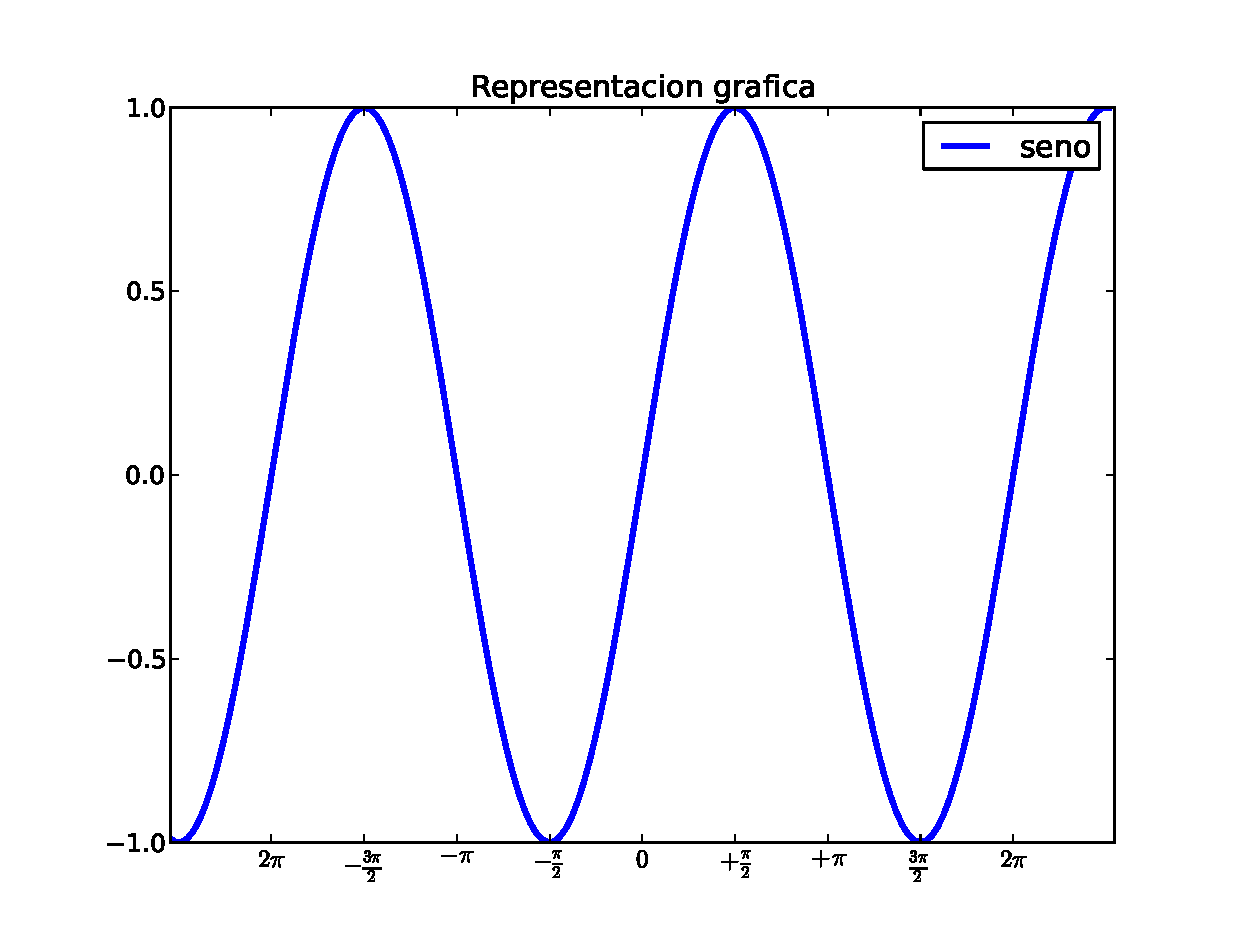
\includegraphics[width=0.75\textwidth]{images/grafi.eps}
\caption{Gr�fica de la funci�n original}
\label{fig:1}
\end{center}
\end{figure}
%------------------------------------------------------------------------------


%------------------------------------------------------------------------------
\begin{table}[!ht]
\begin{center}
\begin{tabular}{|l|c|c|c|c|c|}
\hline
Grado  & Punto c & Punto de Evaluacion & Aproximacion       & Error             & Tiempo CPU           \\ \hline
4      &   0.0   &    1                & 0.833333           & -0.833333         & 0.007406949996948242 \\ \hline
6      &   10    &    5                & 12.4605618963148   & -13.0045830072041 & 0.009202957153320312 \\ \hline
10     &   10    &    10               & -0.544021110889370 & 0                 & 0.010988950729370117  \\ \hline
\end{tabular}
\end{center}
\caption{Tabla de datos obtenidos experimentalmente}
\label{tab}
\end{table}

%------------------------------------------------------------------------------

%++++++++++++++++++++++++++++++++++++++++++++++++++++++++++++++++++++++++++++++
\section{An�lisis de los resultados}
\label{3:sec:4}
\begin{itemize}
\item[$\circ$] Experimento 1:
 Polinomio de taylor de grado 4, punto $c=10.0$.
El punto de evaluci�n ($x$) fue cambiando. A medida que se acercaba al punto $c$, el error fue disminuyendo. La diferencia del tiempo de CPU 
es m�nima. 
\item[$\circ$] Experimento 2:
 Polinomio de Taylor de grado 4, punto $x=2.0$
El punto $c$ fue cambiando. Cuando el punto $c$ es 0, tanto el valor de aproximaci�n como el de error son iguales pero de signos opuestos. 
Si el valor otorgado a $c$ se encuentra lejos de $x$ el error es mayor. 

\item[$\circ$] Experimento 3: 
 Polinomio de Taylor de grado 10, punto $c=10.0$.
El punto $x$ que est� m�s alejado del punto $c$ contien el mayor valor de error. 
En $x=5$ el tiempo de CPU es mayor que en el resto de experimentos realizados. 

\item[$\circ$] Experimento 4:
 Polinomio de Taylor de grado 100, punto $c=-1.0$. 
Se ha cambiado s�lo el n�mero de los decimales de $x$, el error para $x=-0.9$ es menor que el de para 
$x=-0.999999$. 
El tiempo de CPU que se registr� para ambos valores de $x$ contienen una diferencia m�nima. Es le mayor de los tiempos registrados en los 4 experimentos.  

\end{itemize}



%%%%%%%%%%%%%%%%%%%%%%%%%%%%%%%%%%%%%%%%%%%%%%%%%%%%%%%%%%%%%%%%%%%%%%%%%%%%%%%
\chapter{Conclusiones}
\label{chapter:conclusiones}

%%%%%%%%%%%%%%%%%%%%%%%%%%%%%%%%%%%%%%%%%%%%%%%%%%%%%%%%%%%%%%%%%%%%%%%%%%%%%
% Chapter 4: Conclusiones y Trabajos Futuros 
%%%%%%%%%%%%%%%%%%%%%%%%%%%%%%%%%%%%%%%%%%%%%%%%%%%%%%%%%%%%%%%%%%%%%%%%%%%%%%%

 Tras la realizaci\'on de varios c\'odigos en lenguaje Python, los cuales constan de diferentes algoritmos implementados que buscan la soluci\'on al 
planteamiento de dichos c\'odigos, se ha conseguido hallar la aproximaci\'on de f(x)=sin(x) mediante el m\'etodo de Taylor, el error establecido y el tiempo de CPU. 
Para poder analizar y comparar los resultados obtenidos se han llevado a cabo distintos experimentos solicitando en cada uno el grado del polinomio de Taylor,
 el punto central c y el punto x. 

\begin{itemize}
\item
Con dichos valores, se puede afirmar que se debe de aumentar el grado del polinomio tantas veces como sea posible, escoger los puntos x y c con la menor distancia 
existente entre ambos y un mayor n\'umero de cifras decimales, se lograr\'a una mejor aproximaci\'on con un margen menor de error.
En el caso de x = c, el teorema de aproximaci\'on no es adecuado porque solo estaremos calculando la imagen de la funci\'on en el punto c y no una 
aproximaci\'on a la funci\'on.


\item
Al analizar los datos del tiempo de CPU se concluye que al programa Python le toma m\'as tiempo realizar las operaciones con un polinomio de grado 10 que con 
uno de grado 4. Con esto se peude afirmar que cuanto mayor sea el grado del polinomio a calcular m\'as demorar\'a en hacer el c\'alculo, aunque nostros no 
puedamos percibir la diferencia ya que se est\'a trabajando con cent\'esimas y mil\'esimas de segundos. 

\end{itemize}


%%%%%%%%%%%%%%%%%%%%%%%%%%%%%%%%%%%%%%%%%%%%%%%%%%%%%%%%%%%%%%%%%%%%%%%%%%%%%%%

%%%%%%%%%%%%%%%%%%%%%%%%%%%%%%%%%%%%%%%%%%%%%%%%%%%%%%%%%%%%%%%%%%%%%%%%%%%%%%%
\newpage{\pagestyle{empty}\cleardoublepage}
\thispagestyle{empty}
\begin{appendix}

\chapter{Programa en Python}
\label{appendix:1}

\section{Algoritmo principal}
\label{Apendice1:XXX}

\begin{center}
\begin{footnotesize}
\begin{verbatim}

PROGRAMA PRINCIPAL

#!/src/bin/python
#!encoding: UTF-8 
import math 
from sympy import *
import modulo
import time

numero = int(raw_input("Introduzca el grado que desea que 
tenga el Polinomio de Taylor: "))
centro = float(raw_input("Introduzca el punto central donde desea que se evalue el 
Polinomio de Taylor: "))
x = float(raw_input("Introduzca el punto x donde desea 
evaluar el Polinomio de Taylor: "))

modulo.taylor1(x, numero, centro)

\end{verbatim}
\end{footnotesize}
\end{center}

\section{Algoritmo del m�dulo}
\label{Apendice1:YYY}

\begin{center}
\begin{footnotesize}
\begin{verbatim}
/#!/src/bin/python

import math
from sympy import *
import time

def factorial(numero):
  factorial = 1
  while(numero > 1):
    factorial = factorial * numero
    numero = numero - 1
  return factorial
  
\end{verbatim}
\end{footnotesize}
\end{center}
  
\begin{center}
\begin{footnotesize}
\begin{verbatim}

def taylor1(x, numero, centro):
  inicio = time.time()
  c = Symbol('c')
  f = sin(c)
  func = f.evalf(subs={c: centro})
  suma = func
  for i in range (1,numero + 1):
    f_i = diff(f, c)
    v = f_i.evalf(subs={c: centro})
    s= (v / factorial(i)) * ((x - centro) ** i)    
    suma = suma + s
    f = f_i
  error = func - suma
  print 'El valor de la funcion original sin(%f) es igual a %f ' % (centro, func)
  print 'El Polinomio de Taylor de grado n=%d en el punto centro c=%f 
  evaluada en el punto x=%f es igual a %f' % (numero, centro, x, suma)
  print 'El Error de la funcion original con el Polinomio de Taylor es: error=%f' % error
  l=[numero, centro, x, suma, error]
  f = open("Taylor.tex", 'a')
  
\end{verbatim}
\end{footnotesize}
\end{center}

\begin{center}
\begin{footnotesize}
\begin{verbatim}
  f.write('Grado del Polinomio (n) Punto Central (c)  Punto de Evaluacion (x)  
  Aproximacion
  Error Tiempo CPU \n ')
  fin = time.time()
  tiempo_total = fin - inicio
  l=l+[tiempo_total]
  f.write(str(l))
  f.write("\n")
  f.close()
  f=open("Taylor.tex","r")
  print(f.read())
  f.close()
  return taylor1
  
\end{verbatim}
\end{footnotesize}
\end{center}


\chapter{Explicaci�n del programa en Python} 
\label{appendix:2}

\section{Explicacion del Algoritmo}
\label{Apendice2:label}

\begin{center}
\begin{footnotesize}
\begin{verbatim}
En el programa principal primero, importamos las 
librerias que usaremos mas adelante con el comando import o from xxx import yyy 
para importar un elemento concreto de la libreria.
Luego, pedimos por pantalla las 3 variables necesarias para ejecutar 
nuestro programa que son:
el grado del polinomio de Taylor (numero), el punto central (centro) 
y el punto donde se desea evaluar (x). 
Finalmente, acabamos el programa llamando a la funcion taylor1 
que se encuentra en nuestro modulo.

Por ultimo, definimos y1 e y2 para que se evalue la funcion y2 en el rango de la variable y1
y luego que se cree y guarde en el archivo grafico.png.
\end{verbatim}
\end{footnotesize}
\end{center}

\section{Explicacion del algoritmo del modulo}
\label{Apendice2:label2}

\begin{center}
\begin{footnotesize}
\begin{verbatim}

Al igual que en el programa principal, importaremos las librerias 
que utilizaremos posteriormente. 
Primeramente, definimos la funcion factorial, que luego sera usada 
en la otra funcion para calcular el polinomio de Taylor. factorial(numero) 
crea un bucle for que incremente su valor, 
dependiendo de la variable numero introducida.
 
\end{verbatim}
\end{footnotesize}
\end{center}

\begin{center}
\begin{footnotesize}
\begin{verbatim}
La siguiente funcion taylor1 dependera de las tres variables que se han 
introducido por pantalla.

Primero, declaramos una variable c sobre que la que se derivara luego la funcion f 
respecto de ella

Evaluamos la funcion f en el punto c = centro y con ese valor 
inicializamos la variable suma. Luego, entramos en un bucle for, 
en el que se vaya derivando la funcion f y asi, se vaya evaluando en el punto c = centro
para calcular una nueva variable s, propia del polinomio de Taylor,
y asi ir incrementando la variable suma.
 
Ahora calculamos el error cometido entre la funcion original 
y la aproximacion del polinomio de Taylor. 
Seguidamente, mostramos por pantalla los datos obtenidos en el programa 
y creamos una lista l que luego usaremos para escribir en un fichero.
 
Lo siguiente sera parar el cronometro del programa 
y calcular el tiempo total que ha tardado en realizarse.
 
Por ultimo, abrimos un fichero de nombre Taylor.tex 
que actualice lo que hemos obtenido como resultados, 
si no se encuentra ya en el fichero ("a"), 
luego escribimos un encabezado, para saber que significa cada dato 
que luego escribiremos en una única línea con f.write(str(l)).
 
Finalizamos el modulo con un f.close() para cerrar el fichero 
y mostramos por pantalla dicho fichero para comprobar los resultados.
 
\end{verbatim}
\end{footnotesize}
\end{center}


\end{appendix}

%%%%%%%%%%%%%%%%%%%%%%%%%%%%%%%%%%%%%%%%%%%%%%%%%%%%%%%%%%%%%%%%%%%%%%%%%%%%%%%
\addcontentsline{toc}{chapter}{Bibliograf�a}
\bibliographystyle{plain}


\bibliography{bib/references}
\nocite{*}

%%%%%%%%%%%%%%%%%%%%%%%%%%%%%%%%%%%%%%%%%%%%%%%%%%%%%%%%%%%%%%%%%%%%%%%%%%%%%%%

\end{document}
